%%%%%%%%%%%%%%%%%%%%%%%%%%%%%%%%%%%%%%%%%%%%%%%%%%%%%%%%%%%%%%%%%%%%%%%%%%%%%%%%%%%%%%%%%%%%%
%%									Chapitre 1											%
%%%%%%%%%%%%%%%%%%%%%%%%%%%%%%%%%%%%%%%%%%%%%%%%%%%%%%%%%%%%%%%%%%%%%%%%%%%%%%%%%%%%%%%%%%%%%
\chapter{An Overview of the Thesis}\label{chap:intro}
	\citationChap{
	The thing about quotes on the internet is that you can not confirm their validity
	}{Abraham Lincoln}
	\minitoc
	\newpage

%%%%%%%%%%%%%%%%%%%%%%%%%%%%%%%%%%%%%%%%%%%%%%%%%%%%%%%%%%%%%%%%%%%%%%%%%%%%%%%%%%%%%%%%%%%%%



% Début du chapitre

The purpose of this thesis is to provide a summary of the main research line of my PhD work carried out in between October 2017 and March 2021. During my PhD, I was hosted at the Inria Lille-Nord Europe (France) research center, in the SequeL team (now becomes Scool team). I was fortunate to be advised by Dr. Michal Valko, and also co-supervised by Dr. Emilie Kaufmann. The research thematic of SequeL lies in sequential decision making problems, to which all my contributions are devoted. In particular, this document mainly investigates sequential decision making in optimization problems.

\section{Context of the Thesis}\label{sec:intro.context}
	
\subsection{What do we study and why?}\label{sec:intro.context.what}

Imagine that we dispose a simulator for some complex numerical task. Being considered as a black box, we can only get useful information by calling the simulator with different inputs. The goal is to find an input that optimizes the performance of the simulator. In the context of this thesis, we model such a scene as the so-called \gls{sequential optimization}\footnote{We thus do not consider parallelization in this thesis.} problem where a learner sequentially feeds inputs to an environment (the simulator in the previous example) and from which they receive (deterministic or stochastic) feedback/payoffs/rewards/observations\footnote{Those terms can be interchangeably employed.}. After a certain period of trial, the learner shall be able to output a guess for the optimal input. Under some circumstances, a single interaction with the environment could be extremely costly. It is therefore of great interest to carefully choose the input at each time step based on past observations.

Sequential optimization in a stochastic environment is an active research topic in both applied mathematics and computer science communities. For example, the planning problem in a \gls{mdp}, upon which the recent breakthrough of game intelligence of Go~\citep{silver2016alphago} is constructed, is closely related to sequential optimization. Precisely, given the current state of the game, the game intelligence is designed to maximize a certain value function, whose (noisy) observations can be obtained by exploring well-chosen trajectories.

Another example, which is also one important driving force that motivates this thesis originally, is \gls{hpo} of machine learning classifiers. Modern machine learning algorithms often contain many nuisance parameters that cannot be learned through the learning process, but instead, need to be manually specified. Tuning those so-called \gls{hyper-parameters} is often considered as the most tedious part in a data science task. It is hence appealing to design HPO algorithms that automates the process of choosing those hyper-parameters. HPO can be viewed as a BBO problem where function evaluations are supposed to be very expensive. Typically, a function evaluation in HPO involves running the primary machine learning algorithm to completion on a large and high-dimensional dataset, which often takes a considerable amount of time or resources.

Besides, sequential optimization can also serve as an abstraction of numerous real-world problems. To name a few of them, we can think of (risk-averse) portfolio selection problems in finance~\citep{ziemba2010}, designing effective treatment allocation strategies in medicine~\citep{durand2018contextual}, free-energy minimization in chemical engineering or protein structure prediction~\citep{floudas2000}, metamodelling for engineering design optimization~\citep{wang2007}, parameter estimation (inverse problem) of nonlinear dynamic biochemical pathways~\citep{moles2003}, mesh distortion in material science~\citep{charpagne2019ebsd}, and way more. 

Mathematically speaking, an environment is simply a target function to be optimized. This function can be \textbf{discrete or continuous}. In this thesis, we are in particular interested in optimization of functions for which \textbf{none (or few)} regularity assumptions are made, and only \textbf{noisy (or stochastic)} function evaluations (interactions with the environment) can be observed.

%Le problème de planification dans un Processus de Décision Markovien (MDP pour Markov Decision Process, [1]), pouvant modéliser la gestion de ressources dans un système de type smart grids ou encore le contrôle d'un robot, et celui de la construction d'intelligences artificielles pour des jeux, sont très liés à celui de l'optimisation séquentielle puisqu'ils reviennent à déterminer l'action qui dans un état donné maximise une fonction valeur, dont on peut obtenir des réalisations bruitées en explorant des trajectoires bien choisies.

%In this context, since one does not make extra regularity assumptions on the target function, one can imagine that it can be very costly to evaluate the function. Thus a good strategy for choosing adaptively the next observation is needed in order to find an optimal (or quasi-optimal) point with as few number of evaluations as possible. This is the sequential optimization problem. That being said, the main problematic of my thesis is the \emph{global sequential optimization} problem. Several applications could be investigated in this thesis, in particular the \emph{automatic hyper-parameter tuning} of machine learning algorithms~\citep{samothrakis2013,hoffman2014bayesgap,jamieson2016hyperband,li2017hyperband}.

\subsection{How do we approach the problem?}\label{sec:intro.context.how}

Sequential optimization problem has been widely inspired by the literature of~\gls{mab}. The original MAB problem is first studied by~\cite{thompson1933}, and can be described in the following way: A learner is given a \emph{finite} set of $K$ arms and a time horizon $T$. Pulling an arm leads to a stochastic reward that follows some \emph{unknown} distribution underpin that arm. At each time step, the learner can choose to pull one of the arms and observes a reward sampled from its corresponding underlying distribution.

% \begin{remark}\label{remark:partial}
% \begin{leftbar}[remarkbar]
% Note that rewards of unchosen arms at each time step are not revealed: this partially observable feedback setting is thus a special case of the online learning with experts setting.
% \end{leftbar}
% \end{remark}

In its original form, the objective of a MAB learner is to maximize the total rewards in the long run. A natural observation is that, the learner is required to simultaneously acquire new information for potential future well-being (exploration), and optimize the current decision based on past observations (exploitation). This trade-off is stated as the \gls{exploration-exploitation dilemma}. 
%The usual performance criterion of the learner is measured by the total loss of the chosen arm at each time step w.r.t the best arm, namely the \emph{cumulative regret}. Typical good learners like \UCB~\citep{auer2002ucb} trade off between exploration and exploitation. 

However, exploitation does not necessarily provide meaningful incentives in some real applications. Typically, in the previous working examples presented in Section~\ref{sec:intro.context.what}, we do not really care about the potential losses incurred during the whole learning phase. Indeed, we only aim at finding the (near-)optimum of the target function quickly. In this context, it is more natural to assess the learner in an optimization fashion. This setting, often named as \gls{bai}, is thus more closely related to what we are to investigate in this thesis.

\begin{remark}
\begin{leftbar}[remarkbar]
More generally, we talk about \gls{pure exploration} problems~\citep{bubeck2011pure} instead of BAI, where the learner is supposed to gain as much information about the bandit model regardless of rewards. BAI is merely a particular instance of pure exploration, for which the learning objective is to find the optimal arm. Other learning objectives also exist, like finding arms that surpass some pre-defined threshold (see e.g.~\citealt{locatelli2016thresholding}). However, we mostly focus on BAI in this thesis since it is sufficiently representative.
\end{leftbar}
\end{remark}

\subsection{From multi-armed bandits to reinforcement learning}\label{sec:intro.context.rl}

\begin{figure}[ht]
    \centering
    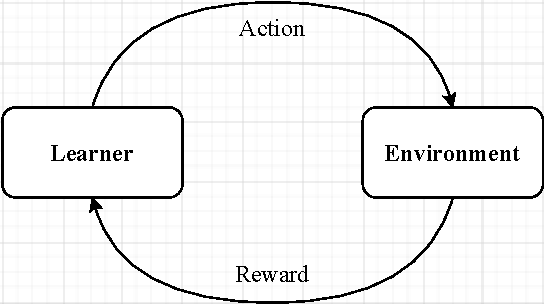
\includegraphics[width=0.33\textwidth]{Chapter1/img/mab.pdf}
    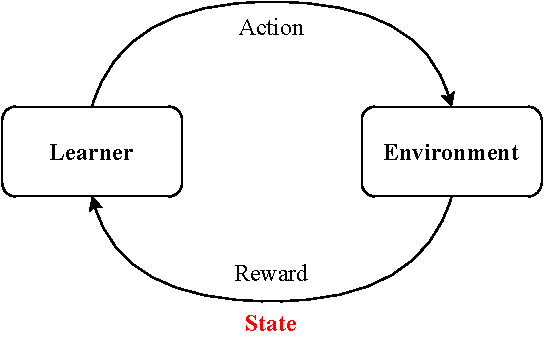
\includegraphics[width=0.33\textwidth]{Chapter1/img/rl.pdf}
    \caption{Left: a bandit learning cycle vs. Right: a reinforcement learning cycle.}
    \label{fig:intro.comparison}
\end{figure}

\section{Multi-Armed Bandits and Optimization}\label{sec:intro.mab}
    
This thesis tries to address sequential optimization problems under stochastic environments from a bandit point of view. A stochastic environment refers to an environment from which stochastic feedback are acquired when an input is queried from the search/action space\footnote{Those terms can be interchangeably employed.} $\mathcal{X}$. Formally, and without loss of generality, we aim to maximize\footnote{Minimization is obviously the same problem.} a target function $f:\mathcal{X}\rightarrow\mathbb{R}$, i.e. find 
\begin{equation}\label{eq:optim}
    \argmax_{x\in\cX} f(x)
\end{equation}
based on a sequence of function values of $f$. Obviously without any prior information on the target function and/or the search space $\cX$, it is just a find-a-needle-in-a-haystack mission. This thesis studies several particular instances of \eqref{eq:optim} with various search spaces and/or different (regularity) assumptions on the target function though, and brings both novel theoretical and practical insights. 

Before jumping into details, we provide a brief overview of different settings investigated in this thesis in this section. More thorough discussion on the problem formulation, in particular how do we assess the performance of algorithms under different settings is given in Chapter~\ref{chap:mab}.

%In its simplest form where the action space $\mathcal{X}$ is finite, the problem can be modeled as a \emph{stochastic multi-armed bandit}. The term \emph{bandit} is named, by analogy, after slot machines (or one-armed bandits) in a casino. A \emph{sequential decision making} problem comes up then when facing with several slot machines (multi-armed bandits). Concretely, a stochastic bandit is a collection of $K$ actions (also called arms) $\mathcal{X} = \{x_1,\ldots,x_K\}$. Each time the learner chooses one action $x_{a_t}\in\mathcal{X}$ which is then fed to the environment. The environment generates a reward $r_{a_t,t}=r_t$ which is assumed to be drawn from an unknown $[0,1]$-valued distribution $\nu_{a_t}$ and is revealed to the learner.

%In its original formulation, the learning objective of a stochastic bandit is to maximise the total reward $\sum_{t=1}^T r_t$ obtained within a given time horizon $T$. In the literature of bandit, we usually denote by $\mu_k$ (resp. $\mu^\star$) the expectation of the unknown distribution $\nu_k$ (resp. the optimal arm), and the previous reward maximisation objective is equivalent to minimising the \emph{cumulative regret}: $T\mu^\star-\sum_{t=1}^T \mu_{a_t}$. %A such learning objective requires the learner to simultaneously acquire new information for potential future well-being (called \emph{exploration}), and optimize the current decision based on past observations (called \emph{exploitation}). 
%Multi-armed bandits naturally addresses the trade-off between exploration and exploitation.

\subsection{Best-arm identification for stochastic multi-armed bandits}\label{sec:intro.mab.bai}

The first setting of interest consists of a finite and one-dimensional search space $\mathcal{X} = \{x_1,x_2,\cdots,x_K\}$. Assume that the underlying reward distribution of arm $x_k$ is characterized by its mean $\mu_k\in\R$, the target function $f$ can be simply interpreted as a mapping form each arm to its mean. The learner then aims to find
\begin{align}\label{eq:optim_bai}
    \argmax_{k\in[K]} \mu_k\,
\end{align}
given some stopping condition. This is the best-arm identification for stochastic multi-armed bandits. Several learning objectives exist for a general BAI problem, among which we are in particular interested in the setting of which the goal is to identify the best arm with high confidence based on a minimum of function evaluations. This is the \gls{fixed-confidence setting} for whom the formal definition, along with those for other learning objectives, are provided and discussed later in Chapter~\ref{chap:mab}.

Existing methods for BAI for stochastic MAB often requires construction of complicated confidence intervals of the mean estimates. We opt for Bayesian machinery to address this problem in this thesis, which is based on the famous Thompson sampling (\TS). \TS is a Bayesian algorithm well known for the classical reward maximization objective, for which it is now seen as a major competitor to the popular \UCB-typed approaches~\citep{auer2002ucb}. A natural question to ask is whether Bayesian methods can be also a good competitor to classical BAI approaches constructed upon complicated confidence intervals. However, it is well known that straight application of \TS cannot yield optimal performance for BAI both in a practical and theoretical point of view. More precisely, it cannot achieve an asymptotic \gls{sample complexity} that matches the lower bound provided by~\cite{garivier2016tracknstop}. Such property is called \gls{asymptotic optimality} that we shall give formal definition later in Chapter~\ref{chap:mab}. An adaptation such as \TTTS proposed by~\cite{russo2016ttts} is needed: by choosing between two different candidate arms in each round, it enforces the exploration of sub-optimal arms, which would be under-sampled by vanilla \TS due to its objective of maximizing rewards. 

In this thesis, we revisit \TTTS both in theory and in practice, trying to provide new insights on its convergence and complexity, and also improve its computational performance.

\subsection{Extension to best-arm identification for linear bandits}\label{sec:intro.mab.linear}

Beyond the previous vanilla setting of BAI, a very natural and widely studied extension is to take a finite set of $K$ arms/contexts/features\footnote{Those terms can be interchangeably employed in the context of this thesis.} $\cX=\{\bx_1,\bx_2,\cdots,\bx_K\}\subset\R^d$ as the search space. The reward of each arm under this circumstance is assumed to depend linearly on a \gls{regression parameter} $\btheta$. The target function $f$ therefore can be considered as a mapping from each arm $\bx$ to its linear combination with $\btheta$, and is thus called linear bandits. Precisely, the learner seeks to find
\begin{align}\label{eq:optim_linbai}
    \argmax_{k\in[K]} \btheta^\top\bx_k\,.
\end{align}
The parameter $\btheta$ is of course \emph{unknown} to the learner. This linear contextual setting describes better some real-world scenarios like advertising placement optimization, and therefore often attracts great attention.

Again, we are interested in the fixed-confidence setting. Previous algorithms on this topic only achieve loose sample complexity bound which is linked to the \gls{G-optimality} of experimental design theory (see e.g.~\citealt{pukelsheim2006optimal}). We conjecture that G-optimality does not describe best the complexity of linear bandits BAI, and therefore try to opt for other more appropriate complexities.

One natural research line is then to design asymptotically optimal algorithm. A simple adaptation of \Track~\citep{garivier2016tracknstop} to the linear setting is very likely to be asymptotically optimal, but remains computationally unfavorable. We thus also seek to design computational friendly algorithms. In this thesis, we investigate both Bayesian approach and confidence interval-based algorithms. In particular, we study whether extensions of \TTTS can be asymptotically optimal.
%Unfortunately, they do not seem to be (asymptotically) optimal (work not published yet). Therefore, knowing whether one can find an *optimal* Bayesian approach remains an open problem.

\subsection{Infinitely-armed bandits and black-box optimization}\label{sec:intro.mab.bbo}

Finally, a more general problem is to consider an infinite (probably uncountable) measurable space $\mathcal{X}$, and each arm $x\in\mathcal{X}$ gets its mean reward $f(x)$ through the reward function $f$. We thus recover~\eqref{eq:optim}:
\[
    \argmax_{x\in\cX} f(x)\,.
\]
This is the \gls{go} or \gls{bbo} problem. Sometimes we can also refer to \gls{zo}, in contrast to \emph{first-order optimization} for which gradient-based information is available.

We study the noisy setting in this thesis. Typical approaches to address GO include \gls{bo} (see e.g.~\citealt{brochu2010bayesian}), evolutionary algorithms and hierarchical bandits (see e.g.~\citealt{bubeck2010x}). In this thesis, we focus on hierarchical bandits algorithms. In the literature of bandits, we often refer to \gls{infinitely-armed bandits} or more precisely \gls{continuum-armed bandits}.

Obviously, we can only expect for a \emph{near-optimal} solution under continuum-armed bandits. We thus opt for another performance measure, namely the \gls{simple regret}, which is the difference between the true optimal function value and the function value of our final guess. Simple regret differs from \gls{cumulative regret} which serves as the performance measure for reward maximization. Formal definitions are provided later in Chapter~\ref{chap:mab}.

In this thesis, we explore the possibility of designing parameter-free hierarchical-bandit algorithms with minimum (smoothness) assumptions.

%In a recent work of ours, we provide a general wrapper for hierarchical bandit algorithms that only have guarantees for their simple regret~\cite{shang2019adaptive}. We show that with a cross-validation scheme, any hierarchical bandit algorithm with simple regret guarantees can be plugged into our meta-algorithm with only a tiny increase in the resulting simple regret.

\subsection{Hyper-parameter optimization}\label{sec:intro.mab.hpo}

Finally, we turn our attention to a more practical question: hyper-parameter optimization. As introduced in Section~\ref{sec:intro.context.what}, efficient hyper-parameter tuning could be of great importance for machine learning practitioners. As is stated, HPO can be naturally modelled as a sequential optimization problem.

The search space of HPO can be both discrete (categorical variables, integer-valued variables, etc) and continuous (real-valued variables). It is natural to ask if hierarchical-bandit algorithms are able to achieve competitive performances for HPO against classical BO algorithms.

Additionally, inspired by a recent BAI-based algorithm \Hyperband~\citep{li2017hyperband}, we seek to propose other BAI-based algorithms for HPO. Indeed, \Hyperband is constructed upon an elimination-based BAI algorithm and achieves state-of-the-art performances compared to previous methods. We, on the other hand, are interested in whether Bayesian algorithms like \TTTS can also be adapted to tackle HPO problems. Note that \TTTS is only designed for \gls{finitely-armed bandits}, an appropriate workaround is hence needed.

\section{A Summary of the PhD}\label{sec:intro.contributions}

From Section~\ref{sec:intro.mab} we can see that the entire thesis is dedicated to one single problem -- sequential bandit optimization -- only with different settings. The full journey of my PhD is, however, far beyond the scope of the present manuscript. This thesis is by no means intended to introduce all the results I have obtained, but rather tell a story about the bandit optimization research line. 

The purpose of this section is to provide a summary of the contributions included in this thesis, and also list all the other work I have participated to just for the record.

\subsection{Summary of the contributions in this thesis}\label{sec:intro.contributions.summary}

We can summarize the contributions presented in this thesis as listed below.

\begin{itemize}[label=\ding{43}]
    \item \cite{shang2020t3c} revisits a Bayesian BAI algorithm \TTTS, and provides new theoretical understandings on its posterior convergence.
    \item \cite{shang2020t3c} also shows that \TTTS achieves asymptotic optimality on the sample complexity.
    \item \cite{shang2020t3c} further proposes a computational improvement \TCC of \TTTS, whilst keeping the same guarantees.
    \item \cite{degenne2020game} proposes a new linear bandits BAI complexity, and provides a comprehensive comparison of existing complexities.
    \item In an unpublished work, we propose several different extensions of \TTTS and \TCC to the linear setting. Unfortunately, we show empirically that they are not asymptotically optimal. In the meantime, \cite{degenne2020game} develops a saddle-point approach that leads to optimal algorithms \LG and \LGC.
    \item \cite{shang2019adaptive} proposes a general wrapper \GPO, using a cross-validation scheme, that wraps up all hierarchical bandit algorithms with simple regret guarantees.
    \item \cite{shang2018adaptive} shows that \HCT is a valid underlying algorithm for \GPO as well as \POO by~\cite{grill2015poo}.
    \item \cite{shang2019dttts} designs a robust and dynamic algorithm \DTTTS based on \TTTS, and shows that such Bayesian-flavored algorithms can be good candidates for applications like hyper-parameter optimization.
    \item \cite{shang2020dttts} provides some further understandings of \DTTTS.
\end{itemize}

\subsection{List of publications and other work}\label{sec:intro.contributions.list}

\paragraph{List of papers (peer-reviewed publications or preprints) included in this thesis.}

\begin{itemize}[label=\ding{171}]
    \item Gamification of pure exploration for linear bandits. In Proceedings of the 37th International Conference on Machine Learning (ICML), 2020.~\citep{degenne2020game}
    \item Fixed-confidence guarantees for Bayesian best-arm identification. In Proceedings of the 23rd International Conference on Artificial Intelligence and Statistics (AIStats), 2020.\citep{shang2020t3c}
    \item Simple (dynamic) bandit algorithms for hyper-parameter optimization. Preprint, 2020.~\citep{shang2020dttts}
    \item A simple dynamic bandit algorithm for hyper-parameter tuning. In 6th Workshop on Automated Machine Learning at International Conference on Machine Learning (ICML-AutoML), 2019.~\citep{shang2019dttts}
    \item General parallel optimisation without a metric. In Proceedings of the 30th International Conference on Algorithmic Learning Theory (ALT), 2019.~\citep{shang2019adaptive}
    \item Adaptive black-box optimisation got easier: HCT needs only local smoothness. In 14th European Workshop on Reinforcement Learning (EWRL), 2018.~\citep{shang2018adaptive}
    \item Hierarchical bandits for black-box optimization and Monte-Carlo tree search. Master Thesis, 2017.~\citep{shang2017master}
\end{itemize}

\paragraph{List of papers (peer-reviewed publications or preprints) not included in this thesis.}

The list below presents other work that are not included in this thesis since they do not really fit in with the scope of the main story line.

\begin{itemize}[label=\ding{171}]
    \item Safe best-arm-identification in linear bandits. Preprint, 2021.~\citep{shang2021safe}
    \item UCB momentum Q-learning: Correcting bias without forgetting. In Proceedings of the 38th International Conference on Machine Learning (ICML), 2021.~\citep{menard2021ucbmq}
    \item Stochastic bandits with vector losses: Minimizing infinite norm of relative losses. Preprint, 2020.~\citep{shang2020vector}
\end{itemize}

\paragraph{Open source software.}

\begin{itemize}[label=\ding{171}]
    \item rlberry - A reinforcement learning library for research and education. Github Repository, 2021.~\citep{rlberry2021}
\end{itemize}

\section{Organization of the Thesis}\label{sec:intro.organization}

We conclude this chapter by providing an outline of the main text of the thesis. 

We start by an introductory Chapter~\ref{chap:mab} about the MAB model. The purpose of this chapter is to present the MAB problem in a more formal way. We first recall some basic notions as well as some fundamental results for stochastic MAB. We then focus on how different best-arm identification/global optimization settings previously mentioned in Section~\ref{sec:intro.mab} are formulated from a bandit point of view.

Chapter~\ref{chap:t3c} is dedicated to the problem of stochastic best-arm identification, where we study in particular Bayesian approaches. This chapter is based on the results presented by~\cite{shang2020t3c}.

Chapter~\ref{chap:lgc} studies best-arm identification for linear bandits. We first investigate the problem from a Bayesian point of view based on some unpublished work. Besides, we also present some general results of linear bandits BAI~\citep{degenne2020game}. 

Chapter~\ref{chap:gpo} is dedicated to continuum-armed bandits. This chapter is mainly based on the results presented by~\cite{shang2018adaptive} and~\cite{shang2019adaptive}.

We talk about one important application of previous problem settings in Chapter~\ref{chap:dttts}, namely \gls{automated machine learning}. We focus especially on hyper-parameter optimization. This chapter is partly based on the results by~\cite{shang2019dttts,shang2020dttts}, but also includes some discussion from my master thesis~\cite{shang2017master}.

Finally, we conclude the present manuscript by some general discussions as well as some future perspectives in Chapter~\ref{chap:conclusion}.

% \newpage
% \bibliographystyle{plain}
% \bibliography{library}
